\chapwithshorttitle{Contexte et acteurs}{Le projet C-ADER : contexte et acteurs}{Le projet C-ADER : contexte et acteurs}

Il est fondamental de définir d'abord le cadre de production des données et le contexte afin de bien comprendre les enjeux du projet.

    \section{Le projet C-ADER, entre science et patrimoine}
        \subsection{Une problématique : conservation des avions et corrosion}

Si la conservation des collections est une des missions premières des professionnels du patrimoine, il s’agit parfois d’une tâche complexe. En effet, certains matériaux constitutifs des œuvres sont instables dans des conditions atmosphériques standards. C’est le cas notamment des métaux, présents dans presque toutes les collections archéologiques, d’objets d’art ou techniques, très sensibles à la corrosion atmosphérique. Ainsi, dans les musées scientifiques et techniques, l'aluminium est très présent. Le Musée de l'Air et de l'Espace du Bourget possède l'une des plus importantes collections d'aéronefs en vraie grandeur retraçant l'histoire de l'aviation ; or, les alliages d'aluminium utilisés sont souvent très sensibles à la corrosion.\\

L'aluminium pur est naturellement protégé contre la corrosion par une fine couche d'oxyde d'aluminium (Al$_2$O$_3$). Cependant, les alliages d’aluminium, spécialement ceux de la série 2XXX utilisés en aéronautique, ne sont pas insensibles à la corrosion. Ces alliages contiennent des impuretés et des éléments d’addition en solution solide et sous forme de composés intermétalliques qui vont générer des défauts. Ces hétérogénéités sont la source de phénomènes de corrosion localisés tels que : la corrosion galvanique, la corrosion par piqûre, la corrosion intergranulaire, la corrosion feuilletante.\\

Par conséquent, les conditions de conservation d’un avion jouent un rôle important dans son processus de corrosion. Il s'agit de trouver les conditions optimales pour exposer et entreposer des appareils généralement de très grandes dimensions (l'envergure d'un avion peut atteindre jusqu'à une vingtaine de mètres), dont les composants sont fragiles, qu'ils soient en bois, en toile ou en métal, et dont les formes hétéroclites ne facilitent pas le stockage, afin qu’ils connaissent la dégradation la plus lente possible. L’exposition des collections aéronautiques au public implique également d’y apporter un soin supplémentaire.\\

A l’heure actuelle, au Musée de l’Air et de l’Espace, un grand nombre d’aéronefs sont exposés en extérieurs ou dans de grands hangars. Dans certains d'entre eux, les variations de température et d’humidité sont importantes et ne peuvent pas être contrôlées. Les matériaux constitutifs des aéronefs sont donc soumis à des alternances de cycles humidification/séchage de plus en plus marquées, provoquant une accélération de la dégradation des matériaux et en particulier des alliages d’aluminium. Or, l’aluminium est très sensible et nécessite un contrôle constant voire de la maintenance pour éviter qu’il ne se dégrade. Les avions qui en sont intégralement constitués font ainsi l’objet d’observations continue.\\

Afin de proposer aux professionnels du patrimoine, conservateurs et restaurateurs, des outils de diagnostic et de conservation pour garantir la conservation à long terme des aéronefs constitués d’alliages d’aluminium, exposés en extérieur ou dans des conditions environnementales non contrôlées, le projet C-ADER (2023-2026), déposé par le Centre de Recherche et de Restauration des Musées de France / Institut de recherche Chimie Paris, le Musée de l’Air et de l’Espace, l’Institut Jean Lamour / Université de Lorraine et l’Institut de Soudure, lauréat de l’appel à projet 2022 de l’Agence Nationale de la Recherche vise à développer des outils d’examen non destructifs basés sur l'utilisation d'ondes guidées non linéaires pour l'analyse et le suivi des structures des avions et des outils de protection contre la corrosion.

        \subsection{Etat de l'art et apport du projet C-ADER  pour les conservateurs et spécialistes du patrimoine}

Jusque-là, les techniques de détection de la corrosion de l’aluminium sur site consistent en une inspection visuelle de l’objet, puis la mise en œuvre de techniques non destructives comme les ultrasons et la radiographie. Des outils spéciaux sont utilisés pour mesurer la couche protectrice de l’aluminium (l’oxyde), à savoir l’interférométrie optique, la spectroscopie IR ou UV-visible. Des techniques sont enfin utilisées pour voir à l’intérieur du métal et y détecter des fissures : il s’agit de méthodes avancées non-destructives comme les ultrasons et la radiographie. Enfin, l'analyse électrochimique évalue les processus de corrosion en surface et aide à comprendre comment l'aluminium se corrode (à quelle vitesse, dans quel milieu).\\

Malheureusement ces techniques ne permettent pas le
plus souvent de détecter des niveaux de dégradation à un stade précoce. Le projet C-ADER cherche justement à développer les techniques de diagnostic de corrosion de l’aluminium à ce stade. La solution retenue dans le cadre du projet est la technologie des ondes ultrasonores guidées\footnote{Pour une définition précise, voir \gls{OUG}}. Des ondes ultrasonores se propagent dans l'épaisseur des matériaux à densité faible sur une certaine distance. Si des fissures ou des piqûres se sont formées dans le métal, la propagation est perturbée et signale le problème.  La particularité et l’efficacité de cette technique repose sur le fait qu’elle permettrait d’analyser les zones où la corrosion n’est pas visible à l’œil nu, comme l’intérieur d’une aile, ou des plaques de tôles très épaisses dans lesquelles la corrosion peut se développer à l’intérieur. Le second avantage de cette technique est qu’elle pourrait détecter la corrosion à un niveau microscopique. De plus, puisque les ondes peuvent se déplacer sur de longues distances avec peu de perte d'énergie, cette technique permettrait d'inspecter de grandes sections de matériau.\\ 

En parallèle, des outils de protection contre la corrosion sont développés en suivant deux axes de recherche. Le premier axe est dédié à la formulation de nouveaux inhibiteurs de corrosion dits « intelligents » et non toxiques, susceptibles de traiter à la fois les parties corrodées et non corrodées ainsi que les zones internes difficiles d'accès. Le second axe concerne la mise en œuvre de techniques de protection cathodique pour protéger les alliages d'aluminium corrodés et assurer une protection anticorrosion à long terme ainsi qu’une maintenance plus aisée.

    \section{Collaboration au sein du projet}
        \subsection{Présentation du consortium et de ses objectifs}

Pour réaliser ces objectifs, un consortium composé de cinq acteurs, l’Institut de recherche Chimie Paris / Centre de Recherche et de Restauration des Musées de France (IRCP / C2RMF), le Musée de l’Air et de l’Espace, l’institut Jean Lamour et l’institut de Soudure s’est formé. Ces différentes institutions possèdent des expertises diverses et complémentaires qui sont indispensables afin de mener à bien ce projet de recherche intrinsèquement multidisciplinaire.
        
        \subsection{Rôle des membres dans la production des données}

Deux grandes tendances se dégagent de ce consortium : une patrimoniale et une autre scientifique, tendances qui influent drastiquement sur le contenu des données traitées.

            \subsubsection{Le Musée de l'Air et de l'Espace}

Le Musée de l’Air et de l’Espace (MAE) est l'acteur principal de ce projet. Situé en France sur le site de l’aéroport Paris-Le Bourget, premier aéroport d'affaires européen, il est placé sous la tutelle du Ministère des Armées. Ce musée centenaire conserve environ 39 000 objets. La collection d'avions du Musée de l'Air et de l'Espace, qui comprend plus de 400 appareils, se distingue par une importante proportion d'avions métalliques, principalement recouverts de surfaces en aluminium peint, dont une partie significative est exposée en plein air. Récemment, le MAE a instauré une politique ambitieuse de conservation-restauration en créant un département dédié, composé d'une équipe de 20 personnes, incluant des gestionnaires, des experts en conservation préventive, des responsables de maintenance et des restaurateurs, sous la direction d'un conservateur spécialisé dans la préservation du patrimoine technique et industriel. Ce projet constitue une opportunité pour le musée d'améliorer ses pratiques de préservation grâce à une meilleure compréhension de l'état de conservation des avions et des processus de dégradation spécifiques à ce type de patrimoine. L'équipe du projet comprend des conservateurs, des restaurateurs, ainsi qu'un ingénieur et des techniciens aéronautiques. Il convient de noter que le musée est le propriétaire des avions soumis à l’étude des processus de corrosion, ce qui le place dans une position privilégiée pour fournir des représentations 3D et détenir des données historiques et techniques essentielles à l'avancement du projet et à la réalisation du jumeau numérique. Le rôle du musée est de fournir les informations historiques et techniques préexistantes relatives aux avions du projet, en s'appuyant sur sa documentation et ses archives. Il est le principal fournisseur de données d’analyse concernant les avions, ainsi que de données d’imagerie 3D, combinant ainsi des données historiques, descriptives et scientifiques. Il est également chargé de collecter des informations relatives à des études qui mettent en lien la rapidité de la corrosion et les conditions de conservation de ses bâtiments. 

\subsubsection{L'Institut de recherche Chimie Paris et le Centre de Restauration des Musées de France}

L’Institut de recherche Chimie Paris, lié au Centre de Recherche et de Restauration des Musées de France (IRCP / C2RMF) est le porteur du projet C-ADER, L’ Institut de Recherche de Chimie Paris a été créé le 1er janvier 2014. Mettant l'accent sur une recherche intégrée, de l'amont à l'aval et des fondamentaux aux applications, ses thématiques couvrent un large éventail de domaines de la chimie : de la chimie moléculaire et de la chimie des polymères, à l'énergie, aux matériaux et aux procédés. Une équipe du Ministère de la Culture, issue du C2RMF, a rejoint le projet et a permis la création d'une équipe mixte. Les équipes du C2RMF/IRCP ont travaillé sur les traitements de conversion chimique et électrochimique pour la protection contre la corrosion et sur des traitements de protection axés sur le développement d'inhibiteurs de corrosion respectueux de l'environnement à base de carboxylates, de tanins. Le Centre de recherche et de restauration des Musées de France (C2RMF) a pour mission de mettre en œuvre, en liaison avec les conservateurs responsables des collections, la politique du service des musées de France en matière de recherche, de conservation préventive et de restauration des collections des musées de France, et de constituer et conserver une documentation sur les matériaux, les techniques et la restauration des œuvres des musées. Dans le cadre de ce projet, le partenaire IRCP/C2RMF sera plus particulièrement chargé de la mise au point des nouvelles formulations de solutions inhibitrices non toxiques et de l’évaluation de leur performance sur les aéronefs.

\subsubsection{L'institut Jean Lamour}

L'Institut Jean Lamour (IJL) est un laboratoire de recherche dédié aux sciences des matériaux et des procédés. Il regroupe environ 550 membres, répartis en 24 équipes, dont 300 sont des chercheurs permanents. L'équipe Corrosion et Traitement de Surface (SIRCM -206) se spécialise notamment dans l'analyse des mécanismes de corrosion des métaux et alliages métalliques dans différents environnements, et travaille également sur le développement de méthodes pour prévenir la corrosion. Depuis de nombreuses années, l'équipe SIRCM explore également les traitements de conversion chimique et électrochimique visant à protéger contre la corrosion des aciers, du zinc, du magnésium et des alliages d'aluminium. Ces traitements incluent le développement d'inhibiteurs de corrosion respectueux de l'environnement. L'équipe collabore également avec le Laboratoire d'Archéologie des Métaux (LAM) et le C2RMF pour la conservation préventive des métaux corrodés dans le patrimoine culturel. Ses compétences sont mises à contribution dans le cadre du projet pour examiner des échantillons d’avions et reproduire certaines de leurs caractéristiques sur des éléments en aluminium synthétique appelés mock-ups. Il est important de noter que, bien que le C2RMF et l’IJL utilisent des techniques d’analyse similaires, leurs méthodes et protocoles sont différents. 

\subsubsection{L'Institut de Soudure}

Enfin, l’Institut de Soudure (IS), créé en 1905, est une association à but non lucratif regroupant 140 membres. Il se spécialise dans la recherche et le développement, ainsi qu’à la formation dans les domaines du soudage et des matériaux d'assemblage. Quatre plateformes technologiques, situées dans l'Est de la France sont mises à disposition pour étudier : les technologies de soudage et de fabrication additive, la caractérisation des matériaux, les essais non destructifs, la surveillance de l'intégrité structurelle et l'intelligence artificielle, ainsi que les matériaux composites. Ils travaillent en étroite collaboration avec deux équipes situées à proximité de Paris qui fournissent des conseils d'experts, notamment sur les essais non destructifs et l’analyse des dommages des matériaux). La principale société affiliée (Institut de Soudure Industrie ISI - 900 personnes) a acquis une solide expérience dans le domaine des essais non destructifs appliqués aux avions modernes et a été impliquée dans l'expertise d'avions anciens. Parmi les équipes spécialisées en essais non destructifs, deux se concentrent sur les techniques utilisant les ondes guidées ultrasonores, choisies pour le projet C-ADER. L'une de ces équipes est dédiée à la recherche et au développement, comprenant 4 docteurs experts dans ce domaine, tandis que l'autre se charge des services techniques sur le terrain. En outre, une collaboration avec le professeur Lawrence Jacobs de l'Institut de technologie de Géorgie à Atlanta (États-Unis) est prévue, en tant que professeur invité. Il est l'un des rares pionniers mondiaux dans la technique des ondes guidées non linéaires, qui reste quelque peu nouvelle en France. Des échanges scientifiques et techniques ont déjà commencé avec lui. De plus, l'équipe de Surveillance et d'Intelligence Artificielle sera chargée du développement d'un outil similaire à un jumeau numérique en étroite collaboration avec le Musée de l’Air et de l’Espace. Un ingénieur aéronautique (Pierre PERRUCAUD de l'ISI, en tant que sous-traitant) renforcera les connaissances de l'équipe sur la structure et la construction des avions, et collectera la documentation technique relative au corpus du projet. L’Institut de Soudure est donc chargé de la recherche et du développement de la technique de diagnostic de la corrosion dans le cadre du projet, fournissant des données de nature scientifique.\\ 

La diversité des profils au sein du consortium peut compliquer le processus d'agrégation des données. Chaque acteur se spécialise dans des techniques d’analyse spécifiques ou se concentre sur certains types d’objets. Avec deux partenaires spécialisés dans les sciences « dures », un acteur axé sur le patrimoine et un autre opérant à l’intersection des deux domaines, les données générées par le projet C-ADER présentent une grande diversité qu’il s’agira de prendre en compte lors de la conception de l’outil numérique. 

\clearpage % Force le saut de page

\begin{figure}[H]
    \centering
    \makebox[\textwidth][c]{%
        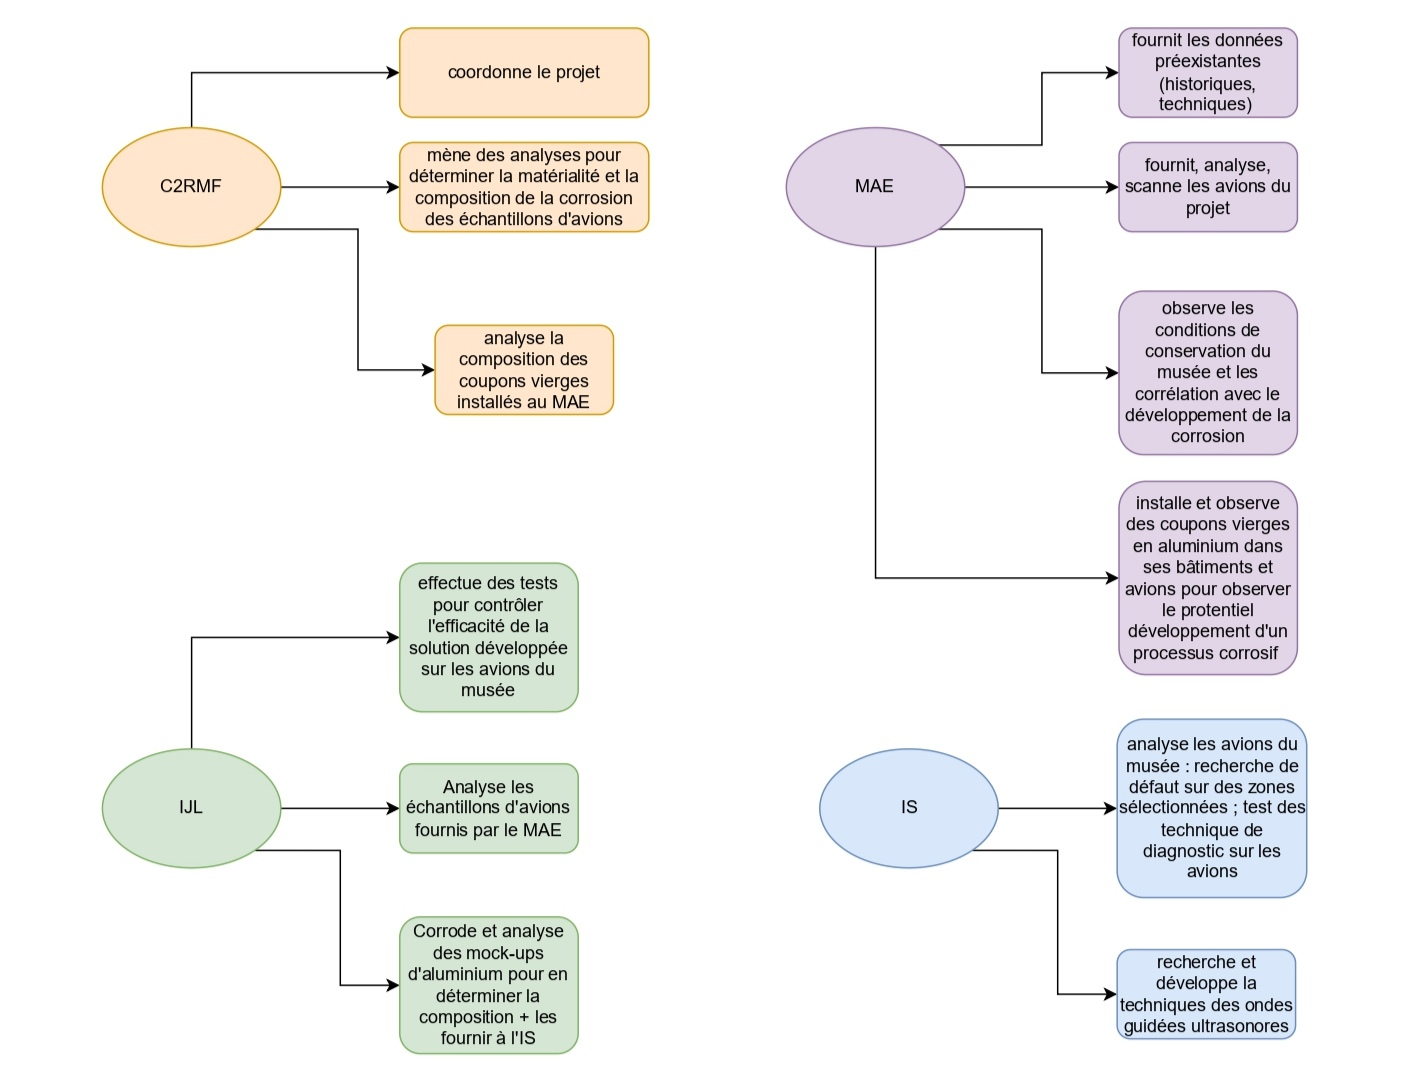
\includegraphics[width=1.4\textwidth, angle=90]{images/roles_des_acteurs.jpg}
    }
    \caption{Le rôle des acteurs du projet C-ADER}
\end{figure}


    \secwithshorttitle{Les objets étudiés}{Les objets étudiés : avions, échantillons, mock-up}{Les objets étudiés : avions, échantillons, mock-up}
    
Les recherches de ce projet seront menées sur plusieurs types d'objets qu’il convient de présenter. Les premiers -et les plus importants- éléments à être analysés sont six avions du Musée de l’Air et de l’Espace. Ces avions sont constitués majoritairement d’alliages 2XXX à base d’aluminium-cuivre contenant des traces de fer et de manganèse, abrégé Al-Cu (Fe-Mn). Ce choix est justifié par la volonté d'étudier des avions aussi bien entreposés en intérieur qu’à l’extérieur, et dont l'état de dégradation est varié. On trouve : 

\begin{itemize}
    \item Deux Boeing 707, le « château de Maintenon » (dont il ne reste plus que l’avant du fuselage) conservés dans un hangar, et le « château de Dampierre », conservé quant à lui dans son intégralité en extérieur, issus tous deux de la flotte des Boeing « Châteaux in the Sky » de la compagnie Air France.
    \item Un Morane Paris, plus précisément un Morane-Saulnier MS. 760 Paris,
    \item Un autre Boeing, mais cette fois-ci un B17G, conservé dans un hangar,
    \item Deux Mirages IV, un conservé en extérieur et très largement corrodé, et un autre conservé en intérieur.
\end{itemize}

L’appareil sélectionné pour la réalisation d’un premier jumeau numérique est le Boeing 707 « Château de Maintenon ». Il convient de préciser que seul le nez de l’appareil ayant été conservé par le musée, sa représentation numérique est susceptible de ne faire figurer que la partie existante actuellement, et non l’intégralité de l’avion. Par sa nature même, cette section est plus accessible pour la réalisation d’analyses, permettant ainsi des prélèvements directs sur le fuselage.\\

Un avion entier n’a pas vocation à être analysé sur place, c'est-à-dire au Musée de l’Air et de l’Espace, par tous les acteurs impliqués dans le projet. Seuls le service restauration et conservation du musée, ainsi que l’Institut de Soudure au début du projet, seront amenés à y travailler, l’objectif pour l’Institut de Soudure étant d’identifier des potentiels défauts présents sur les zones de travail sélectionnées sur chaque avion.\\

Les différents acteurs du projet travailleront dans un premier temps sur des prélèvements -appelés échantillons- provenant de plusieurs avions. Le Centre de recherche et de restauration des musées de France (C2RMF) et l’Institut Jean Lamour (IJL) mèneront de concert des examens afin de caractériser la composition, la morphologie et le niveau de dégradation des échantillons prélevés. À partir des données collectées sur ces derniers des échantillons modèles (mock-up) seront préparés. Ces mock-up constitués d’alliages d’aluminium 2024 seront artificiellement corrodés afin de reproduire les faciès de corrosion observés. C’est sur ces échantillons modèles que seront dans un premier temps testées à la fois les techniques d’analyse non destructive à base d’ondes guidées et les méthodes de protection contre la corrosion. Ces techniques et traitements seront finalement mis en œuvre sur les aéronefs sélectionnés pour validation finale.\\

La connaissance de ces types d’objets et des échanges qui vont s’effectuer entre les différents partenaires sera ainsi essentielle pour l’étude des données produites et la conception des outils de valorisation du projet C-ADER.

\clearpage % Force le saut de page

\begin{figure}[H]
    \centering
    \makebox[\textwidth][c]{%
        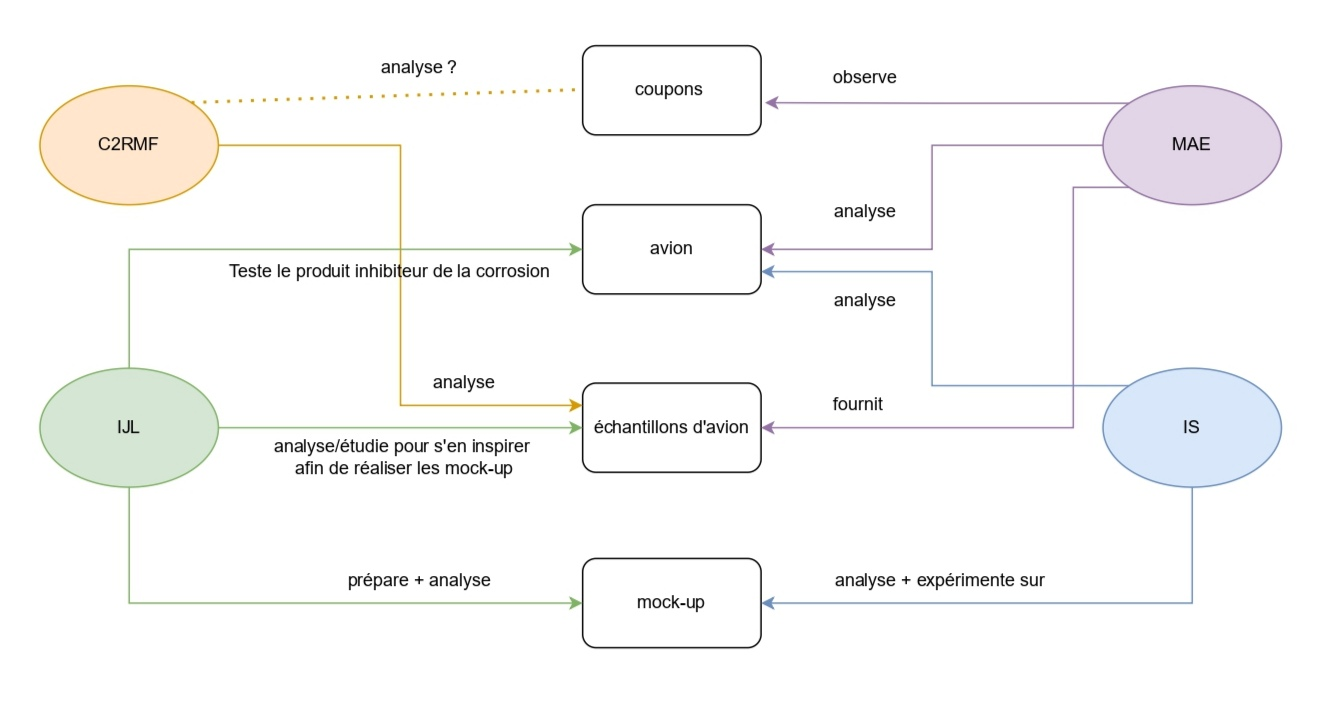
\includegraphics[width=1.4\textwidth, angle=90]{images/objets_etudies.jpg}
    }
    \caption{Les objets étudiés}
    \label{fig:votre_label2_ici}
\end{figure}
